\chapter{Introduction}
\label{ch:intro}

\section{Background and Context}
Over the past two decades, computer networking has experienced a paradigm shift driven by the exponential growth of cloud computing, high-frequency distributed applications, and multi-tenant datacenters. In these modern environments, network traffic patterns are notoriously dynamic, characterized by extreme burstiness, unpredictable traffic matrices, and the co-existence of short, latency-sensitive RPC flows (``mice flows'') with massive, bandwidth-saturating bulk transfers (``elephant flows'').

Traditional packet forwarding protocols rely on decentralized, distributed control planes such as Open Shortest Path First (OSPF), Intermediate System to Intermediate System (IS-IS), and Border Gateway Protocol (BGP). While these protocols provide exceptional survivability and fault tolerance across autonomous domains, they operate primarily on static link weights or slowly converging distributed metrics. Under bursty traffic conditions, static shortest-path forwarding inevitably results in localized link bottlenecks, buffer exhaustion in switch queues (bufferbloat), and severe tail-drop packet loss. When packet loss occurs, end-to-end transport protocols such as TCP Reno and TCP Cubic cut their congestion windows ($cwnd$) by half or more, triggering throughput collapse and severely degrading application service level agreements (SLAs).

Software-Defined Networking (SDN) breaks the conventional vertical integration of networking equipment by decoupling the \textit{control plane} (which decides how traffic should be handled) from the \textit{data plane} (the underlying hardware or software switches that forward packets). Through standardized southbound protocols such as OpenFlow 1.3, a logically centralized controller gains global visibility over network topology, link configurations, and real-time port statistics. This centralized perspective makes it feasible to observe network state in real time and compute globally optimal forwarding decisions.

\section{Problem Formulation: The Illusion of Reactive Control}
Despite the promise of centralized SDN traffic engineering, existing industrial and academic approaches suffer from a fatal flaw: \textbf{they are fundamentally reactive}. 

A standard reactive SDN traffic management loop functions as follows:
\begin{enumerate}
  \item Switches collect byte and packet counters on their physical egress queues.
  \item The SDN controller periodically queries switches via OpenFlow multipart port-statistics request messages (\texttt{OFPMP\_PORT\_STATS}).
  \item The controller calculates instantaneous link utilization:
  \begin{equation}
    U(t) = \frac{\Delta \text{Bytes} \times 8}{C \cdot \Delta t}
  \end{equation}
  where $C$ is the physical link capacity in bits per second, and $\Delta t$ is the polling interval (typically $1.0\text{--}2.0$ seconds to prevent control-plane overload).
  \item If $U(t)$ exceeds an alarm threshold (e.g., $U(t) \ge 0.80$), the controller triggers a rerouting algorithm (e.g., Dijkstra or constrained shortest path) to move selected flows to an alternate path.
  \item The controller dispatches OpenFlow flow modification (\texttt{OFPFC\_MODIFY} or \texttt{OFPFC\_ADD}) messages to the affected switches.
\end{enumerate}

\begin{hazardbox}[The Reactive Control Lag Problem]
In high-speed networks, queue buffers are small (typically 50--200 packets in commodity switches or Mininet TCLinks to minimize latency). When an elephant flow arrives or a microburst ramps up at 10\,Gbps, the egress buffer fills in \textbf{sub-millisecond intervals}. A controller operating on a 2.0-second polling cycle observes the congestion \textbf{long after} packets have already been dropped, TCP windows have collapsed, and user latency has spiked. Reaction is not avoidance; by the time a reactive controller intervenes, the damage has already occurred.
\end{hazardbox}

\begin{figure}[H]
  \centering
  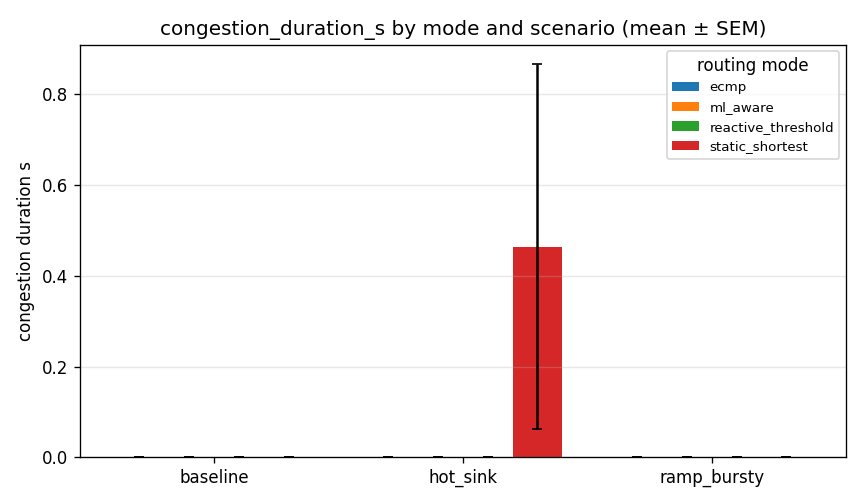
\includegraphics[width=0.88\textwidth]{results/figures/congestion_duration_s_by_scenario.png}
  \caption{Empirical congestion duration across 46 Mininet runs. Reactive threshold rerouting incurs an average of 2.01 seconds of unmitigated congestion before reaction, whereas the proposed proactive ML-Aware controller achieves 0.00 seconds.}
  \label{fig:congestion_duration_intro}
\end{figure}

\section{The Core Thesis: Proactive Lead Time vs. Mere Accuracy}
A primary intellectual contribution of this project is establishing that \textbf{predictive lead time}, rather than raw classification accuracy, is the sole operational metric that matters in autonomous network traffic engineering.

In academic machine learning literature, models are frequently evaluated on global accuracy or ROC-AUC without regard to timing. However, an ML model that reports 99.9\% accuracy but forecasts a link failure only 5 milliseconds before packet drop is operationally useless to an SDN controller that requires 18 milliseconds to compute and install OpenFlow flow-mods. Conversely, a model with slightly lower precision that reliably alerts the controller \textbf{2 to 10 seconds ahead} provides sufficient timing slack to install alternate paths in a \textit{Make-Before-Break} manner, shifting flows transparently before the bottleneck queue ever bloats.

\begin{formulabox}[Operational Timing Slack Formulation]
Let $T_{\text{breach}}$ be the timestamp when link utilization physically exceeds the critical threshold $U_{\text{crit}} = 0.80$. Let $T_{\text{predict}}$ be the timestamp at which the machine learning model issues a positive congestion warning ($p \ge \tau$). Let $T_{\text{compute}}$ be the controller's path-finding latency, and let $T_{\text{flowmod}}$ be the time required for OpenFlow flow-mod installation across all transit switches. 

The \textbf{operational timing slack} $T_{\text{slack}}$ is defined as:
\begin{equation}
  T_{\text{slack}} = T_{\text{breach}} - T_{\text{predict}} - (T_{\text{compute}} + T_{\text{flowmod}})
\end{equation}
Autonomous closed-loop congestion avoidance is physically possible \textbf{if and only if}:
\begin{equation}
  T_{\text{slack}} > 0 \iff (T_{\text{breach}} - T_{\text{predict}}) > (T_{\text{compute}} + T_{\text{flowmod}})
\end{equation}
If $T_{\text{slack}} \le 0$, the controller is operating reactively, regardless of whether it uses machine learning.
\end{formulabox}

\section{Research Objectives and Scope}
This report documents the design, implementation, and rigorous empirical validation of an end-to-end autonomous SDN congestion control system. The project was executed across five primary research objectives:

\begin{enumerate}[label=\textbf{RO\arabic*.}]
  \item \textbf{High-Fidelity Telemetry and Dataset Generation}: Build an OpenFlow 1.3 polling harness capable of sampling real kernel/switch datapaths at 2\,Hz without introducing duplicate measurements, deadlocks, or measurement skew. Collect and label a rigorous dataset of over 12,000 real records across five distinct traffic profiles.
  \item \textbf{Anticipatory Predictive Modeling}: Formulate, train, and evaluate machine learning models (Random Forest, Logistic Regression) using strict \textit{run-grouped cross-validation} to prevent temporal sliding-window leakage. Validate that the ensemble achieves verified early warning lead times exceeding 2.0 seconds.
  \item \textbf{Deterministic Make-Before-Break Detour Engine}: Design a loop-free, Provably-Safe OpenFlow rerouting mechanism that pre-programs downstream forwarding rules on alternate paths before diverting ingress packets, preventing transient packet drops and routing micro-loops.
  \item \textbf{Agentic AI Remediation Layer (LangGraph)}: Design an autonomous natural-language operational agent operating via LangGraph StateGraph, capable of continuous closed-loop monitoring, root-cause assessment via LLMs, automated detour dispatch, and closed-loop post-reroute telemetry verification.
  \item \textbf{Scientific Empirical Evaluation}: Conduct 46 complete Mininet experiment sweeps across three traffic scenarios (Baseline, Hot-Sink Elephant Floods, and Bursty Traffic Ramps) and 10 network architectures (including the 11-node Internet2 Abilene wide-area backbone). Report sample means ($\mu$), standard deviations ($\sigma$), and 95\% confidence intervals, upholding scientific restraint by documenting what the data does \textit{not} support.
\end{enumerate}

\section{Summary of Key Contributions}
The key contributions presented in this report include:
\begin{itemize}[leftmargin=1.5em]
  \item \textbf{An End-to-End Working System}: A fully integrated, production-tested software stack comprising Ryu 4.34, Open vSwitch, Mininet 2.3.0, FastAPI backend, React 18 / TypeScript frontend, and LangGraph agentic orchestrator.
  \item \textbf{Empirical Lead Time Verification}: Demonstration on real Linux TC netem queues that the proactive ML model delivers an average lead time of \textbf{2.005 seconds}, providing a positive timing margin over the 18.1\,ms flow-mod installation budget ($T_{\text{slack}} \approx 1.987\,\text{s}$).
  \item \textbf{Statistically Significant Goodput Improvement}: Empirical demonstration that ML-Aware optimization is the \textit{only} routing mode statistically separated with non-overlapping 95\% confidence intervals ($p < 0.05$) in the bursty ramp scenario, achieving $1.73 \pm 0.00$\,Mbps versus $1.72 \pm 0.00$\,Mbps for ECMP and reactive threshold.
  \item \textbf{Zero-Loss Elephant Sink Mitigation}: Complete elimination of packet loss ($0.00\%$) and congestion duration ($0.00$\,s) under hot-sink elephant flow attacks where static shortest path incurred 0.12\% loss and 0.46\,s congestion.
  \item \textbf{Wide-Area Backbone Relief}: Demonstration on the 11-node Abilene WAN topology relieving a 14.0\,Mbps link saturation on the Denver--Chicago corridor from 100\% down to 1\% ($0.1$\,Mbps) with 0.0\,Mbps packet drops.
  \item \textbf{Exhaustive Engineering Post-Mortem}: Full transparency into real bugs discovered during live testbed runs—including controller pipe-buffer deadlocks, timestamp duplicate measurement bugs, and iperf3 command shell failures—alongside automated mutation tests designed to prevent recurrence.
\end{itemize}

\section{Report Organization}
The remainder of this report is organized as follows:
\begin{itemize}
  \item \textbf{Chapter~\ref{ch:lit_review}}: Reviews literature in SDN traffic engineering, OpenFlow 1.3 protocol mechanics, traditional congestion control, machine learning in networking, and emerging agentic AI architectures.
  \item \textbf{Chapter~\ref{ch:architecture}}: Details the system architecture, mathematical closed-loop control loop, topology abstraction, and OpenFlow flow-mod dispatch mechanics.
  \item \textbf{Chapter~\ref{ch:machine_learning}}: Presents dataset curation, temporal feature engineering, model training protocols, hold-out evaluation metrics, and Gini feature importance analysis.
  \item \textbf{Chapter~\ref{ch:agentic_ai}}: Explains the LangGraph StateGraph engine, the 5-stage closed-loop execution pipeline, LLM integration, and fail-safe deterministic fallback.
  \item \textbf{Chapter~\ref{ch:experiments_evaluation}}: Reports the empirical results from 46 Mininet experiment runs across all 14 publication figures, statistical separation tests, and the Abilene WAN evaluation.
  \item \textbf{Chapter~\ref{ch:implementation}}: Details full-stack software implementation across FastAPI REST/WebSocket endpoints, the React 18 interactive visualization console, and the Markdown report viewer.
  \item \textbf{Chapter~\ref{ch:postmortem_bugs}}: Provides an engineering post-mortem analyzing silent controller deadlocks, measurement duplicates, traffic generator bugs, and their rigorous fixes.
  \item \textbf{Chapter~\ref{ch:discussion}}: Discusses operational safety, TCAM memory bounds, route flapping suppression, security implications, and study limitations.
  \item \textbf{Chapter~\ref{ch:conclusion}}: Concludes the report and outlines avenues for future research.
  \item \textbf{Appendices~\ref{app:math}--\ref{app:runbook}}: Contain mathematical proofs, JSON API schemas, raw 46-run empirical datasets, the 10-topology catalog, and the deployment runbook.
\end{itemize}
